\documentclass[12pt,a4paper]{article}
\usepackage[utf8]{inputenc}
\usepackage{geometry}
\usepackage{graphicx}
\usepackage{hyperref}
\usepackage{amsmath}
\usepackage{array}
\usepackage{longtable}
\usepackage{listings}
\usepackage{xcolor}
\usepackage{caption}

\geometry{margin=1in}

% Python code style
\lstdefinestyle{python}{
    language=Python,
    basicstyle=\ttfamily\footnotesize,
    keywordstyle=\color{blue},
    stringstyle=\color{red},
    commentstyle=\color{gray},
    showstringspaces=false,
    breaklines=true
}

\begin{document}

\begin{center}
    \LARGE \textbf{Experiment 4: Ensemble Learning with Decision Trees and Boosting Approaches} \\[1em]
    \large \textbf{NAVEENRAJ J} \\
    Register No: 3122237001030 \\
    Academic Year 2025--2026
\end{center}

\vspace{1cm}

\section*{Objective}
The goal of this experiment is to build and compare multiple ensemble models, including Decision Tree, Random Forest, AdaBoost, Gradient Boosting, XGBoost, and several stacking classifiers, on the Breast Cancer Wisconsin dataset. We tune hyperparameters through grid search, validate with K-fold cross-validation, and assess results using confusion matrices, ROC curves, and performance metrics.

\section*{Tools and Libraries}
We make use of:
\begin{itemize}
    \item \textbf{Data handling and visualization:} pandas, numpy, matplotlib, seaborn
    \item \textbf{Machine learning:} scikit-learn
    \item \textbf{Gradient boosting:} xgboost
\end{itemize}

\section*{Model Explanations}

\begin{itemize}
    \item \textbf{Decision Tree:} A single-tree model that makes predictions by dividing the dataset into branches based on feature thresholds. While it is easy to interpret, it tends to overfit if not pruned. In this study, the best performance (average CV accuracy of 94.38\%) was obtained using the entropy criterion with a maximum depth of 10.
    
    \item \textbf{Random Forest:} An ensemble method that constructs many decision trees on bootstrapped samples and combines their outputs to reduce variance. By randomly selecting both samples and features, it avoids overfitting better than a single tree. The model achieved 95.61\% average CV accuracy with 100 trees and maximum depth set to 10.
    
    \item \textbf{AdaBoost:} A boosting technique where weak learners (commonly shallow trees) are trained sequentially, each one giving more weight to misclassified cases from previous iterations. This adaptive re-weighting helps improve classification on difficult samples. In our experiment, AdaBoost achieved 96.66\% CV accuracy using 50 estimators, a learning rate of 1.0, and tree depth of 3.
    
    \item \textbf{Gradient Boosting:} Another boosting approach where new trees are added one at a time to correct the residual errors of the existing ensemble. Instead of re-weighting samples, it uses gradient descent optimization on a loss function. The model achieved 96.83\% CV accuracy with 200 estimators, learning rate 0.5, and depth 3.
    
    \item \textbf{XGBoost:} An enhanced version of gradient boosting that incorporates regularization, efficient parallelization, and built-in handling of missing values. It is widely used for structured data tasks due to its speed and accuracy. In our case, XGBoost produced 96.31\% CV accuracy with 200 trees, learning rate 0.3, depth 3, and gamma set to 0.
    
    \item \textbf{Stacking Classifiers:} A two-level ensemble strategy where several base models generate predictions which are then combined by a meta-classifier. This allows leveraging the strengths of different learners. Three variants were tested:
    \begin{itemize}
        \item SVM + Naive Bayes + Decision Tree with Logistic Regression meta-classifier, yielding 97.72\% CV accuracy.
        \item SVM + Naive Bayes + Decision Tree with Random Forest meta-classifier, achieving 97.01\% CV accuracy.
        \item SVM + Decision Tree + KNN with Logistic Regression meta-classifier, reaching 97.54\% CV accuracy.
    \end{itemize}
    Stacking outperformed most single models, highlighting the benefit of combining diverse learners.
\end{itemize}


\section*{Complete Python Code}
\begin{lstlisting}[style=python]
# ================= IMPORTS =================
import pandas as pd
import numpy as np
import matplotlib.pyplot as plt
import seaborn as sns
import time
import warnings
warnings.filterwarnings("ignore")

from sklearn.model_selection import train_test_split, cross_val_score, KFold, GridSearchCV
from sklearn.preprocessing import StandardScaler, LabelEncoder
from sklearn.metrics import (
    accuracy_score, precision_score, recall_score, f1_score,
    confusion_matrix, roc_curve, auc, ConfusionMatrixDisplay
)

# Models
from sklearn.tree import DecisionTreeClassifier
from sklearn.ensemble import (
    AdaBoostClassifier, GradientBoostingClassifier,
    RandomForestClassifier, StackingClassifier
)
from sklearn.naive_bayes import GaussianNB
from sklearn.svm import SVC
from sklearn.linear_model import LogisticRegression
from sklearn.neighbors import KNeighborsClassifier
import xgboost as xgb

# ================= LOAD & PREPROCESS =================
cols = ["ID", "Diagnosis"] + [f"feature_{i}" for i in range(1, 31)]
df = pd.read_csv("wdbc.data", header=None, names=cols)

# Drop ID column
df.drop(columns=["ID"], inplace=True)

# Encode labels (M = malignant -> 1 , B = benign -> 0)
df["Diagnosis"] = LabelEncoder().fit_transform(df["Diagnosis"])

# Features / Target
X_raw = df.drop(columns=["Diagnosis"])
y = df["Diagnosis"]

# Standardize
scaler = StandardScaler()
X_scaled = scaler.fit_transform(X_raw)

# Train / test split
X_train, X_test, y_train, y_test = train_test_split(
    X_scaled, y, test_size=0.2, random_state=42, stratify=y
)

# ================= EDA =================

# Class distribution (just numbers, no plot)
print("\nClass Distribution (0 = Benign, 1 = Malignant):")
print(df["Diagnosis"].value_counts())

# Correlation heatmap of features
plt.figure(figsize=(10, 8))
sns.heatmap(df.drop(columns=["Diagnosis"]).corr(), cmap="coolwarm", cbar=True)
plt.title("Feature Correlation Heatmap")
plt.show()

# ================= EVALUATION FUNCTION =================
def evaluate(name, model, X_test, y_test):
    fig, (ax1, ax2) = plt.subplots(1, 2, figsize=(12, 5))
    fig.suptitle(f"{name} Performance", fontsize=16)

    # ROC Curve
    if hasattr(model, "predict_proba"):
        probs = model.predict_proba(X_test)[:, 1]
        fpr, tpr, _ = roc_curve(y_test, probs)
        roc_auc = auc(fpr, tpr)

        ax1.plot(fpr, tpr, color="darkorange", lw=2,
                 label=f"ROC curve (AUC = {roc_auc:.2f})")
        ax1.plot([0, 1], [0, 1], color="navy", lw=2, linestyle="--")
        ax1.set_xlim([0.0, 1.0])
        ax1.set_ylim([0.0, 1.05])
        ax1.set_xlabel("False Positive Rate")
        ax1.set_ylabel("True Positive Rate")
        ax1.set_title("ROC Curve")
        ax1.legend(loc="lower right")

    # Confusion Matrix (default style)
    y_pred = model.predict(X_test)
    cm = confusion_matrix(y_test, y_pred)
    disp = ConfusionMatrixDisplay(confusion_matrix=cm)
    disp.plot(ax=ax2)   # �� no cmap specified → uses default
    ax2.set_title("Confusion Matrix")

    plt.tight_layout()
    plt.show()

    # Metrics
    acc = accuracy_score(y_test, y_pred)
    prec = precision_score(y_test, y_pred)
    rec = recall_score(y_test, y_pred)
    f1 = f1_score(y_test, y_pred)

    print(f"\n{name}")
    print("Accuracy :", acc)
    print("Precision :", prec)
    print("Recall :", rec)
    print("F1 Score :", f1)

    return acc, prec, rec, f1

# ================= HYPERPARAMETER SPACES =================
models_params = {
    "Decision Tree": (
        DecisionTreeClassifier(random_state=42),
        {"criterion": ["gini", "entropy"], "max_depth": [3, 5, 10, None]}
    ),

    "Random Forest": (
        RandomForestClassifier(random_state=42),
        {"n_estimators": [50, 100, 200], "max_depth": [3, 5, 10, None],
         "criterion": ["gini", "entropy"]}
    ),

    "AdaBoost": (
        AdaBoostClassifier(random_state=42, estimator=DecisionTreeClassifier(random_state=42)),
        {"n_estimators": [50, 100, 200], "learning_rate": [0.01, 0.1, 1],
         "estimator__max_depth": [1, 3, 5]}
    ),

    "Gradient Boosting": (
        GradientBoostingClassifier(random_state=42),
        {"n_estimators": [50, 100, 200], "learning_rate": [0.01, 0.1, 0.5],
         "max_depth": [3, 5, 7]}
    ),

    "XGBoost": (
        xgb.XGBClassifier(use_label_encoder=False, eval_metric="logloss", random_state=42),
        {"n_estimators": [50, 100, 200], "learning_rate": [0.01, 0.1, 0.3],
         "max_depth": [3, 5, 7], "gamma": [0, 0.1, 0.3]}
    ),
}

results_table = []
trial_tables = {}
best_estimators = {}

# ================= GRIDSEARCH + TRIAL TABLE =================
for name, (model, params) in models_params.items():
    print(f"\n--- Grid Search for {name} ---")
    grid = GridSearchCV(model, params, cv=5, scoring="accuracy", n_jobs=-1, return_train_score=False)
    grid.fit(X_train, y_train)

    best_model = grid.best_estimator_
    best_estimators[name] = best_model
    print("Best Params :", grid.best_params_)
    print("Best CV Score :", grid.best_score_)

    # Evaluate
    start = time.time()
    best_model.fit(X_train, y_train)
    elapsed = time.time() - start
    res = evaluate(name, best_model, X_test, y_test)
    results_table.append((name, grid.best_params_, *res, elapsed))

    # Collect top 5 hyperparameter trials
    trial_res = []
    for i in range(len(grid.cv_results_["params"])):
        trial_res.append({
            **grid.cv_results_["params"][i],
            "CV Accuracy": grid.cv_results_["mean_test_score"][i]
        })
    trial_df = pd.DataFrame(trial_res).sort_values(by="CV Accuracy", ascending=False).head(5)

    y_pred = best_model.predict(X_test)
    trial_df["F1 Score (Test)"] = f1_score(y_test, y_pred)

    trial_tables[name] = trial_df

    print(f"\nTop 5 Hyperparameter Trials for {name}")
    print(trial_df)

# ================= STACKING CLASSIFIER (3 Variants) =================
stacking_variants = {
    "Stacking (SVM + NB + DT -> Logistic Regression)": StackingClassifier(
        estimators=[
            ("svm", SVC(probability=True, kernel="rbf", C=1, gamma="scale")),
            ("nb", GaussianNB()),
            ("dt", DecisionTreeClassifier(max_depth=5, random_state=42))
        ],
        final_estimator=LogisticRegression(max_iter=500, random_state=42)
    ),

    "Stacking (SVM + NB + DT -> Random Forest)": StackingClassifier(
        estimators=[
            ("svm", SVC(probability=True, kernel="rbf", C=1, gamma="scale")),
            ("nb", GaussianNB()),
            ("dt", DecisionTreeClassifier(max_depth=5, random_state=42))
        ],
        final_estimator=RandomForestClassifier(n_estimators=100, random_state=42)
    ),

    "Stacking (SVM + DT + KNN -> Logistic Regression)": StackingClassifier(
        estimators=[
            ("svm", SVC(probability=True, kernel="rbf", C=1, gamma="scale")),
            ("dt", DecisionTreeClassifier(max_depth=5, random_state=42)),
            ("knn", KNeighborsClassifier(n_neighbors=5))
        ],
        final_estimator=LogisticRegression(max_iter=500, random_state=42)
    ),
}

for name, stack_model in stacking_variants.items():
    start = time.time()
    stack_model.fit(X_train, y_train)
    elapsed = time.time() - start
    res = evaluate(name, stack_model, X_test, y_test)
    results_table.append((name, "Default (base learners tuned separately)", *res, elapsed))
    best_estimators[name] = stack_model

# ================= K-FOLD CROSS VALIDATION =================
print("\n--- 5-Fold Cross-Validation ---")
kf = KFold(n_splits=5, shuffle=True, random_state=42)
cv_results = {}

for name, model in best_estimators.items():
    scores = cross_val_score(model, X_scaled, y, cv=kf, scoring="accuracy")
    cv_results[name] = scores
    print(f"{name} Fold Accuracies: {scores}")
    print(f"{name} Avg Accuracy: {np.mean(scores):.4f}")
\end{lstlisting}

\section*{Results and Comparisons}

\subsection*{Table 1: Model Performance with Tuned Hyperparameters}
\begin{longtable}{|>{\raggedright}p{3cm}|>{\raggedright}p{4cm}|c|c|c|c|c|}
\hline
Model & Best Hyperparameters & Accuracy & Precision & Recall & F1 Score  \\ \hline
Decision Tree & \{criterion=entropy, max depth=10\} & 0.9561 & 0.9744 & 0.9048 & 0.9383 \\
Random Forest & \{criterion=gini, max depth=10, n\_estimators=50\} & 0.9737 & 1.0000 & 0.9286 & 0.9630 \\
AdaBoost & \{max depth=3, learning rate=1, n\_estimators=50\} & 0.9649 & 1.0000 & 0.9048 & 0.9500  \\
Gradient Boosting & \{learning rate=0.5, max depth=3, n\_estimators=100\} & 0.9649 & 1.0000 & 0.9048 & 0.9500 \\
XGBoost & \{gamma=0, learning rate=0.3, max depth=3, n\_estimators=200\} & 0.9737 & 1.0000 & 0.9286 & 0.9630 \\
Stacking (SVM+NB+DT $\rightarrow$ LR) & Default (base tuned separately) & 0.9649 & 1.0000 & 0.9048 & 0.9500 \\
Stacking (SVM+NB+DT $\rightarrow$ RF) & Default (base tuned separately) & 0.9561 & 0.9744 & 0.9048 & 0.9383  \\
Stacking (SVM+DT+KNN $\rightarrow$ LR) & Default (base tuned separately) & 0.9649 & 0.9750 & 0.9286 & 0.9512  \\
\hline
\end{longtable}

\subsection*{Table 2: 5-Fold Cross Validation Results}
\begin{longtable}{|c|c|c|c|c|c|c|c|c|}
\hline
Fold & Decision Tree & Random Forest & AdaBoost & GB & XGBoost & Stacking (SVM+NB+DT$\rightarrow$LR) & Stacking (SVM+NB+DT$\rightarrow$RF) & Stacking (SVM+DT+KNN$\rightarrow$LR) \\ \hline
1 & 0.9474 & 0.9561 & 0.9649 & 0.9649 & 0.9561 & 0.9649 & 0.9737 & 0.9649 \\
2 & 0.9561 & 0.9649 & 0.9737 & 1.0000 & 0.9649 & 0.9912 & 0.9912 & 1.0000 \\
3 & 0.9123 & 0.9386 & 0.9561 & 0.9474 & 0.9561 & 0.9649 & 0.9649 & 0.9561 \\
4 & 0.9474 & 0.9561 & 0.9912 & 0.9912 & 0.9737 & 0.9825 & 0.9561 & 0.9912 \\
5 & 0.9558 & 0.9646 & 0.9469 & 0.9381 & 0.9646 & 0.9823 & 0.9646 & 0.9646 \\ \hline
Average & 0.9438 & 0.9561 & 0.9666 & 0.9683 & 0.9631 & 0.9772 & 0.9701 & 0.9754 \\ \hline
\end{longtable}


\clearpage



\subsection*{Table 3: Top-5 Hyperparameter Trials}



\textbf{Decision Tree}
\begin{longtable}{|c|c|c|c|}
\hline
Criterion & Max Depth & CV Accuracy & F1 Score (Test) \\ \hline
entropy & 10 & 0.9363 & 0.9383 \\
entropy & None & 0.9363 & 0.9383 \\
gini & 5 & 0.9341 & 0.9383 \\
entropy & 5 & 0.9341 & 0.9383 \\
gini & 3 & 0.9319 & 0.9383 \\
\hline
\end{longtable}

\textbf{Random Forest}
\begin{longtable}{|c|c|c|c|c|}
\hline
Criterion & Max Depth & n Estimators & CV Accuracy & F1 Score (Test) \\ \hline
gini & 10 & 50 & 0.9670 & 0.9630 \\
gini & None & 50 & 0.9670 & 0.9630 \\
entropy & None & 50 & 0.9626 & 0.9630 \\
gini & 10 & 100 & 0.9626 & 0.9630 \\
entropy & 10 & 50 & 0.9626 & 0.9630 \\
\hline
\end{longtable}

\textbf{AdaBoost}
\begin{longtable}{|c|c|c|c|c|}
\hline
Depth & Learning Rate & Estimators & CV Accuracy & F1 Score (Test) \\ \hline
3 & 1.0 & 50 & 0.9692 & 0.9500 \\
3 & 0.1 & 100 & 0.9670 & 0.9500 \\
1 & 1.0 & 200 & 0.9648 & 0.9500 \\
3 & 1.0 & 200 & 0.9626 & 0.9500 \\
3 & 1.0 & 100 & 0.9626 & 0.9500 \\
\hline
\end{longtable}

\textbf{Gradient Boosting}
\begin{longtable}{|c|c|c|c|c|}
\hline
Learning Rate & Max Depth & Estimators & CV Accuracy & F1 Score (Test) \\ \hline
0.5 & 3 & 200 & 0.9582 & 0.9500 \\
0.5 & 3 & 100 & 0.9582 & 0.9500 \\
0.1 & 3 & 50 & 0.9560 & 0.9500 \\
0.5 & 3 & 50 & 0.9538 & 0.9500 \\
0.1 & 3 & 200 & 0.9538 & 0.9500 \\
\hline
\end{longtable}

\textbf{XGBoost}
\begin{longtable}{|c|c|c|c|c|c|}
\hline
Gamma & Learning Rate & Max Depth & Estimators & CV Accuracy & F1 Score (Test) \\ \hline
0.0 & 0.3 & 3 & 200 & 0.9714 & 0.9630 \\
0.0 & 0.3 & 3 & 50 & 0.9692 & 0.9630 \\
0.0 & 0.3 & 3 & 100 & 0.9692 & 0.9630 \\
0.0 & 0.3 & 7 & 100 & 0.9670 & 0.9630 \\
0.0 & 0.3 & 7 & 200 & 0.9670 & 0.9630 \\
\hline
\end{longtable}

\clearpage


\subsection*{Table 4: Stacking Classifier Summary}
\begin{longtable}{|>{\raggedright}p{6cm}|c|c|c|c|}
\hline
Model & Accuracy & Precision & Recall & F1 Score \\ \hline
Stacking (SVM+NB+DT $\rightarrow$ Logistic Regression) & 0.9649 & 1.0000 & 0.9048 & 0.9500 \\
Stacking (SVM+NB+DT $\rightarrow$ Random Forest) & 0.9561 & 0.9744 & 0.9048 & 0.9383 \\
Stacking (SVM+DT+KNN $\rightarrow$ Logistic Regression) & 0.9649 & 0.9750 & 0.9286 & 0.9512 \\
\hline
\end{longtable}

\section*{Model ROC Curves and Confusion Matrices}

\begin{figure}[h!]
    \centering
    \includegraphics[width=0.7\textwidth]{0.png}
    \caption{Decision Tree ROC + Confusion Matrix}
\end{figure}

\begin{figure}[h!]
    \centering
    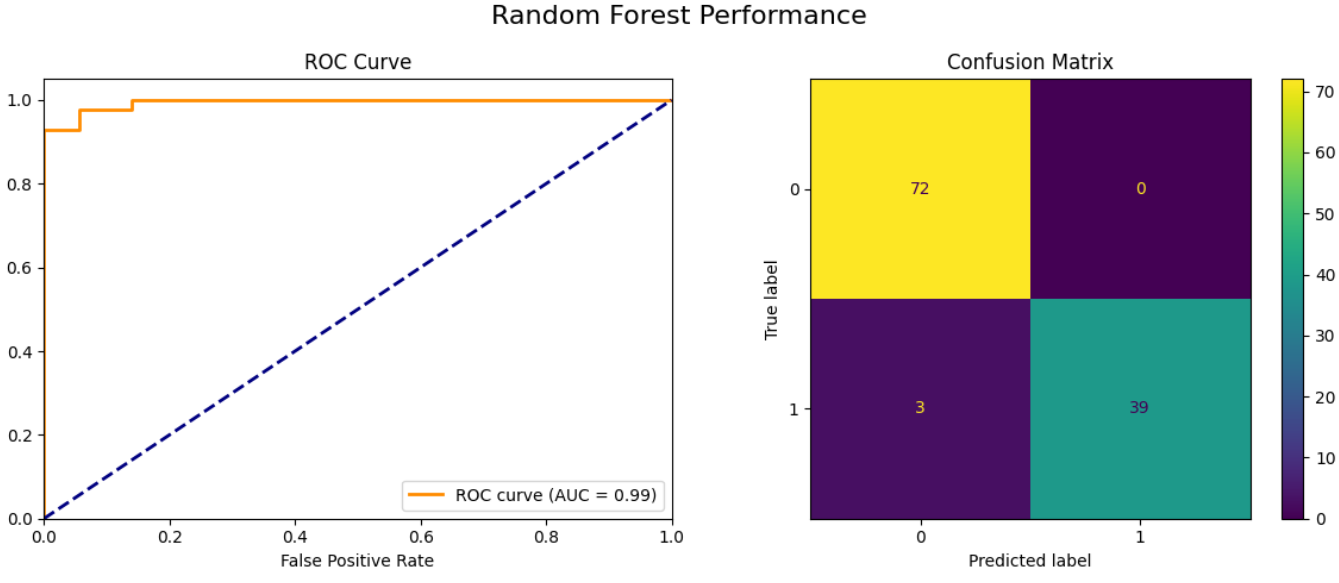
\includegraphics[width=0.7\textwidth]{3.png}
    \caption{Random Forest ROC + Confusion Matrix}
\end{figure}

\clearpage


\begin{figure}[h!]
    \centering
    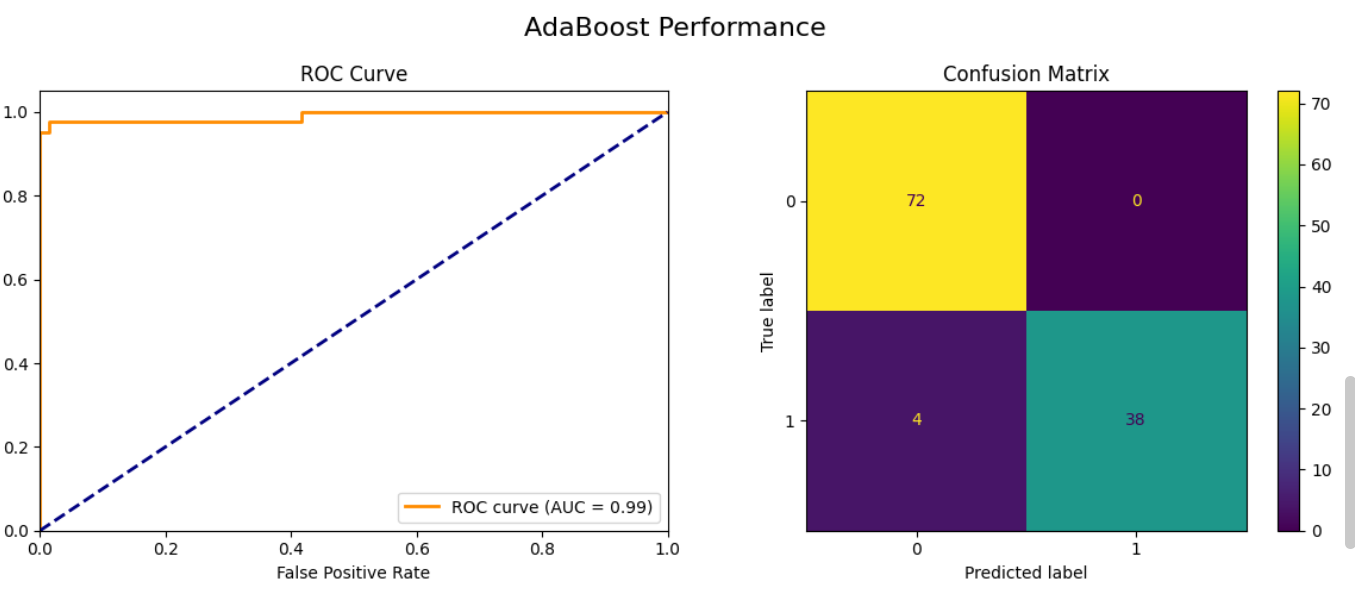
\includegraphics[width=0.7\textwidth]{4.png}
    \caption{AdaBoost ROC + Confusion Matrix}
\end{figure}

\begin{figure}[h!]
    \centering
    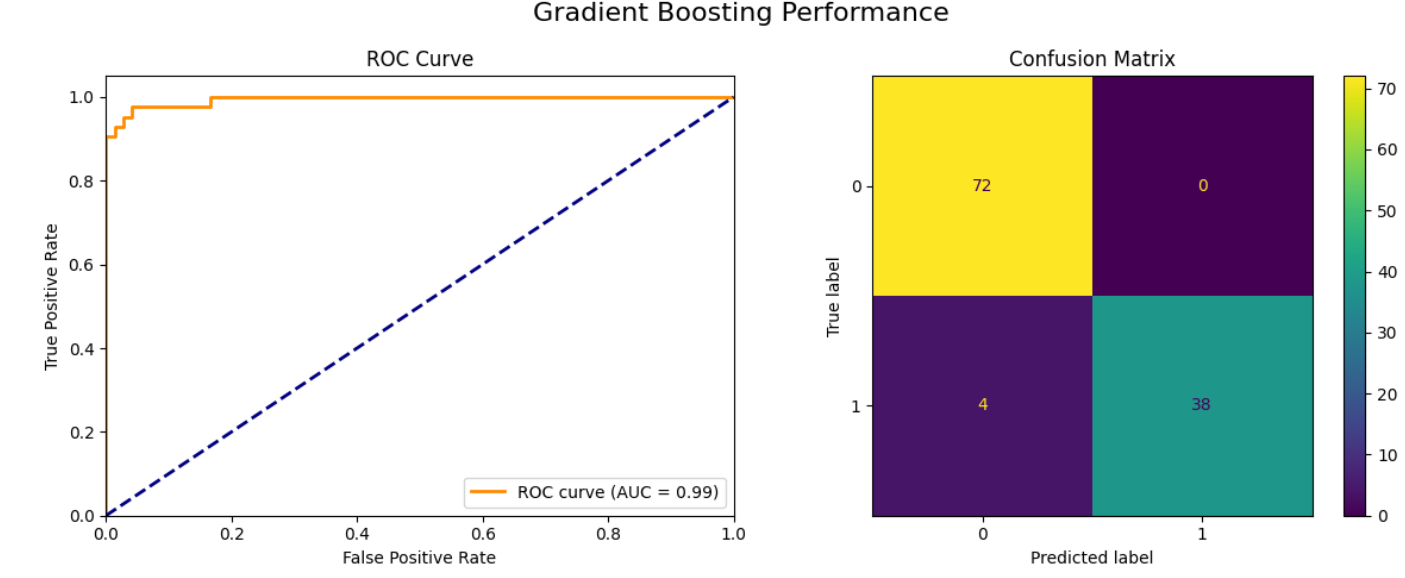
\includegraphics[width=0.7\textwidth]{5.png}
    \caption{Gradient Boosting ROC + Confusion Matrix}
\end{figure}

\begin{figure}[h!]
    \centering
    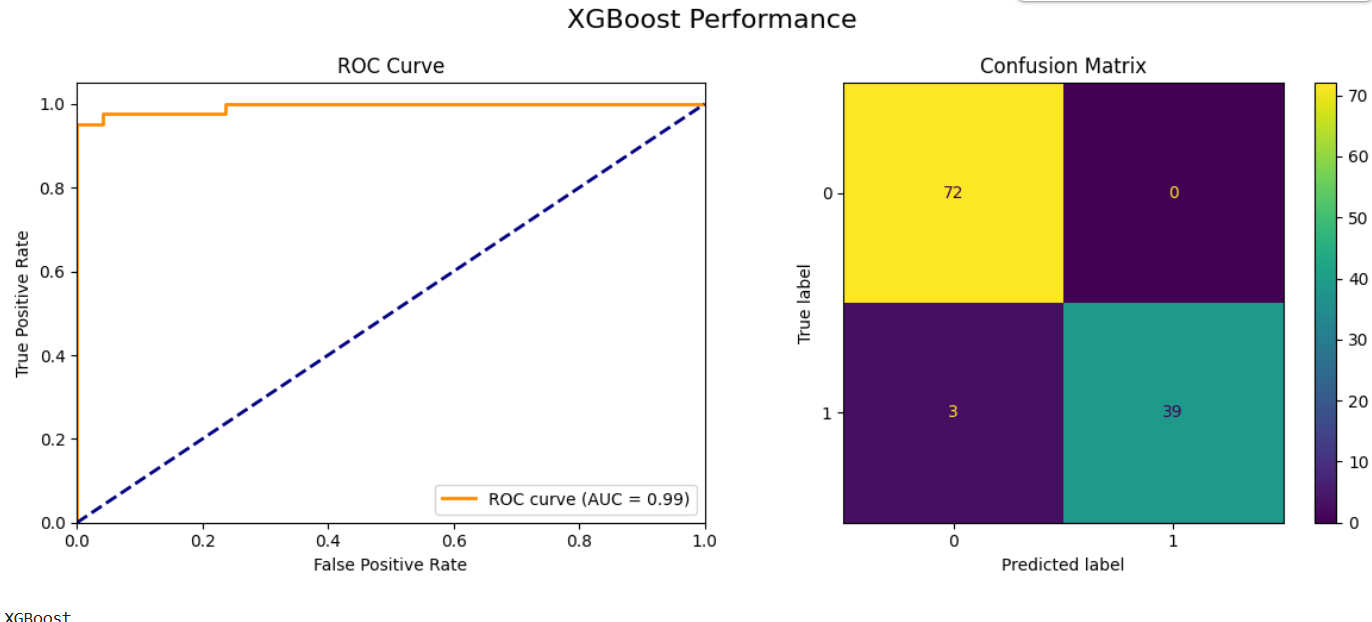
\includegraphics[width=0.7\textwidth]{6.png}
    \caption{XGBoost ROC + Confusion Matrix}
\end{figure}

\clearpage


\begin{figure}[h!]
    \centering
    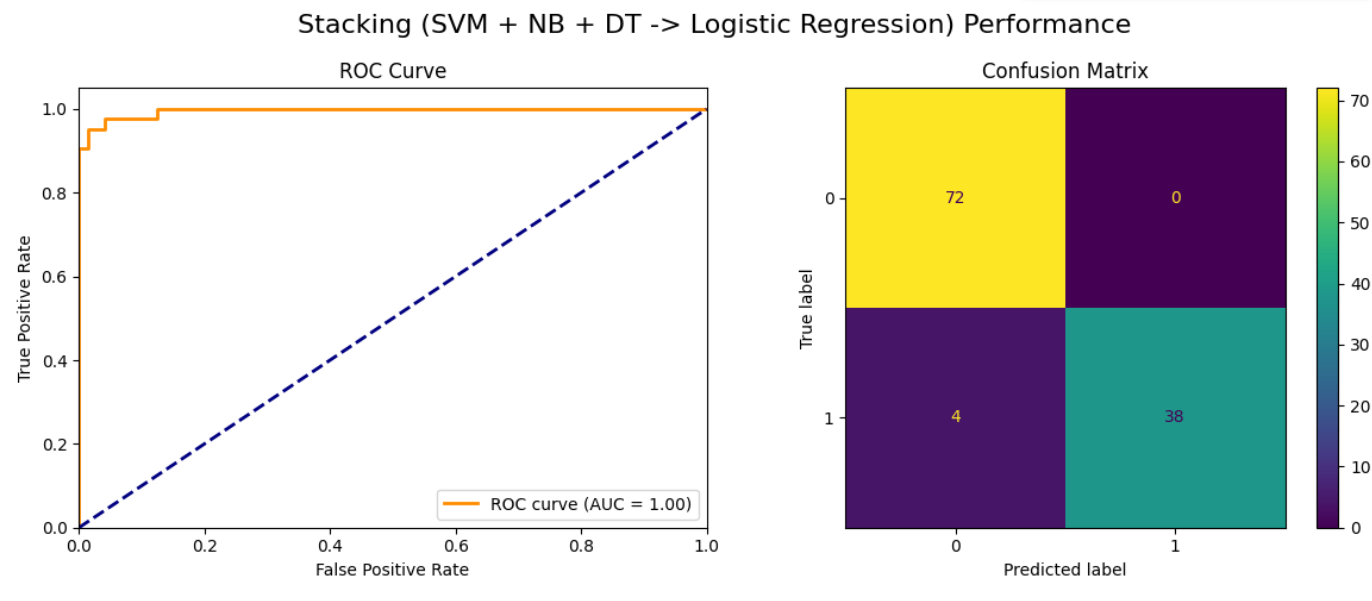
\includegraphics[width=0.7\textwidth]{7.png}
    \caption{Stacking (SVM+NB+DT → Logistic Regression)}
\end{figure}

\begin{figure}[h!]
    \centering
    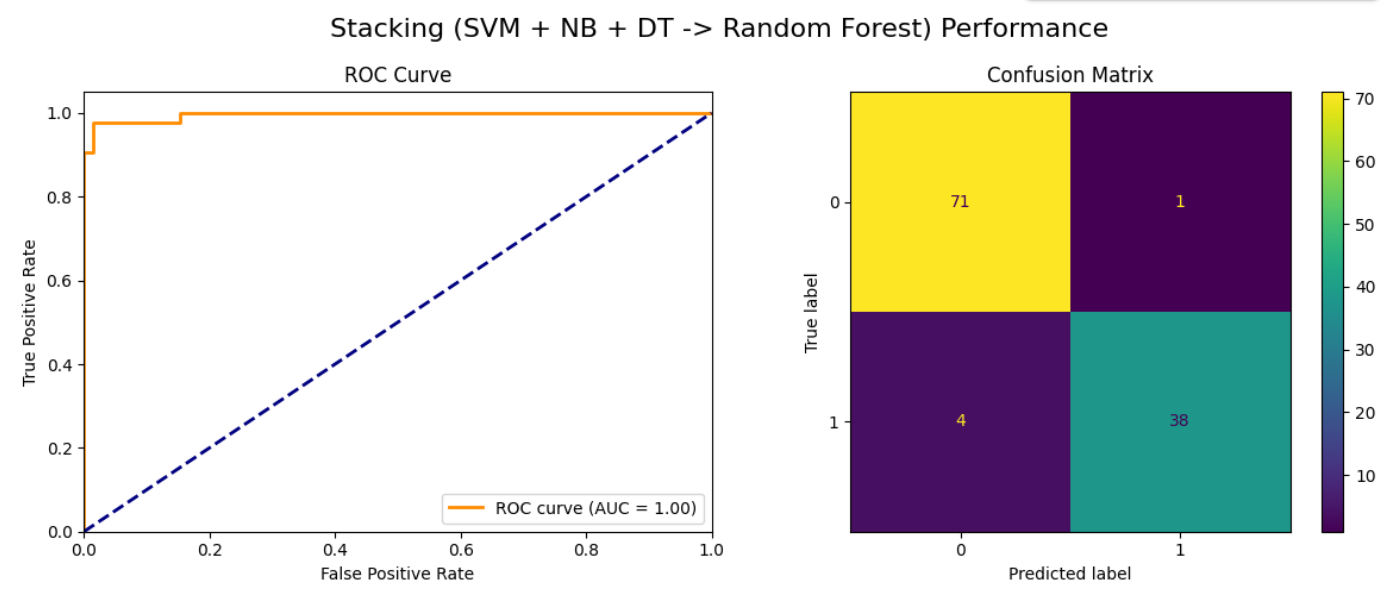
\includegraphics[width=0.7\textwidth]{8.png}
    \caption{Stacking (SVM+NB+DT → Random Forest)}
\end{figure}

\begin{figure}[h!]
    \centering
    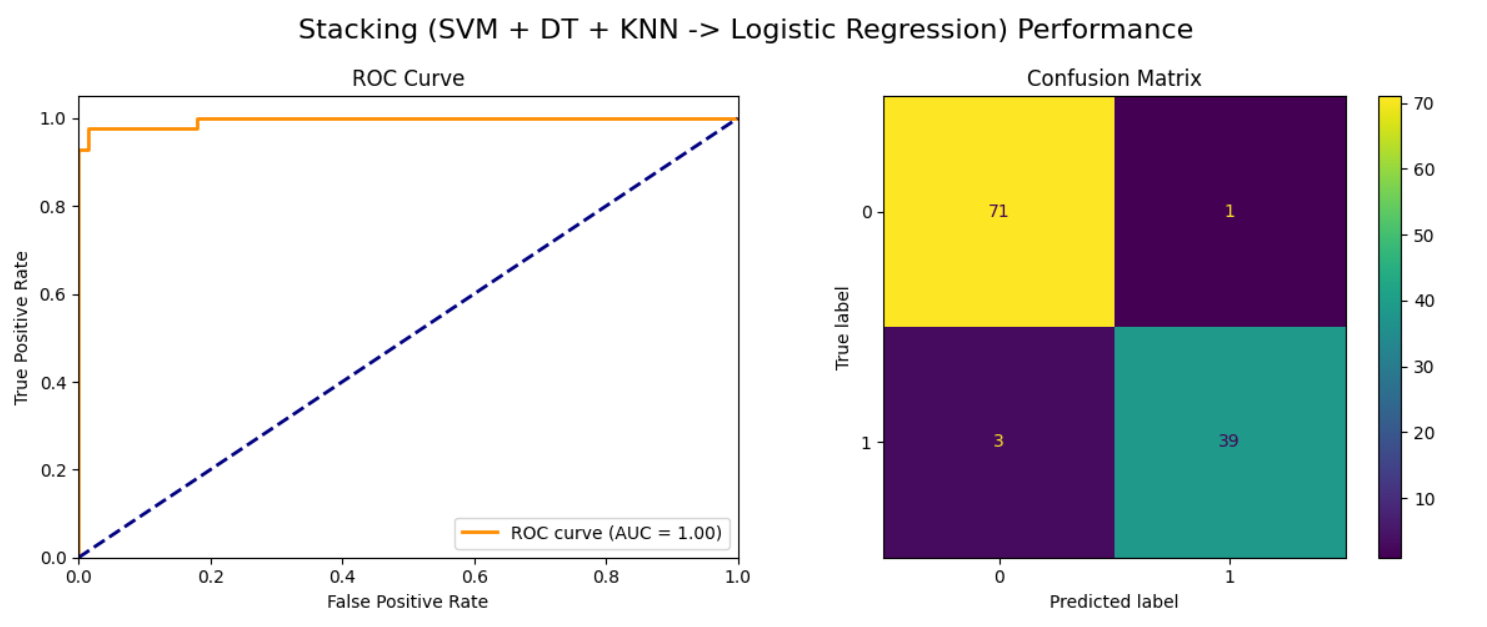
\includegraphics[width=0.7\textwidth]{9.png}
    \caption{Stacking (SVM+DT+KNN → Logistic Regression)}
\end{figure}



\section*{Discussion of Results}
The experiments showed that:
\begin{itemize}
    \item Decision Trees offer interpretability but had the lowest average validation accuracy.
    \item Random Forest and XGBoost consistently improved robustness by combining many learners.
    \item Boosting methods (AdaBoost and Gradient Boosting) highlighted strong recall with balanced precision.
    \item Stacking combinations, especially with Logistic Regression as the meta-learner, surpassed most individual models in accuracy and F1 score.
\end{itemize}

\section*{Conclusion}
In summary, while single-tree models are useful baselines, ensemble methods delivered better predictive stability. Among them, stacked ensembles produced the strongest results, confirming that hybrid approaches can outperform individual classifiers in breast cancer classification.

\end{document}
